\chapter{Background}\label{back}

\lettrine{I}{n} this chapter we explain the main used concepts and tools, related to Agorà; as it has been revealed in the Introduction, this work has been thought for HPC applications that run in parallel architectures, so we start clarifying what are these target systems and how they are built; after that, we explain the concepts of Design Space Exploration and Design of Experiments, that represents the kernel of this work, in union with the idea of application dynamic online autotuning; finally, we present the used tools for the various communications among Agorà components and for applications complete model prediction, highlighting their principal characteristics and features: the Message Queue Telemetry Transport (MQTT) messaging protocol and the Generalized Linear Regression interface by Apache Spark\textsuperscript{TM} Machine Learning MLlib library.

\section{Target architecture}

High Performance Computing applications have complex and massive tasks to do, so they need huge computing power in order to accomplish their objectives.

Parallel computing (\cite{barney2012introduction}) simultaneously uses multiple resources in order to solve a computational problem, taking advantage of concurrency, that is the possibility to execute, at the same time, those parts that are independent each other; in figure \ref{fig::pC::serial} we can see an example of serial computation, with a single processor that executes problem instructions sequentially, one after another; figure \ref{fig::pC::parallel} instead represents a possible parallel computation, where problem is split in four parts that can be executed concurrently on different processors:

\begin{figure}[H]

    \centering

    \subfloat[][\emph{Serial computation}\label{fig::pC::serial}]
        {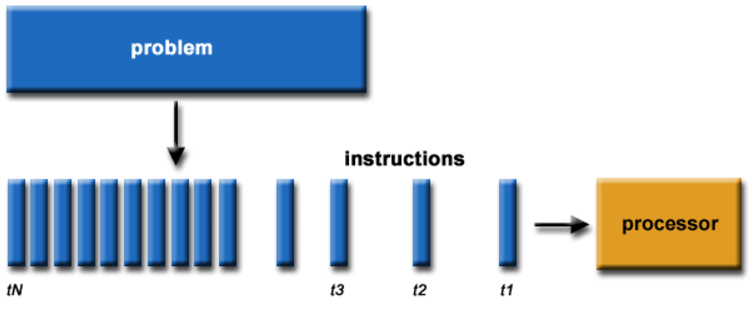
\includegraphics[width = 0.45\textwidth]{ser_prob}}
    \quad
    \subfloat[][\emph{Parallel computation}\label{fig::pC::parallel}]
        {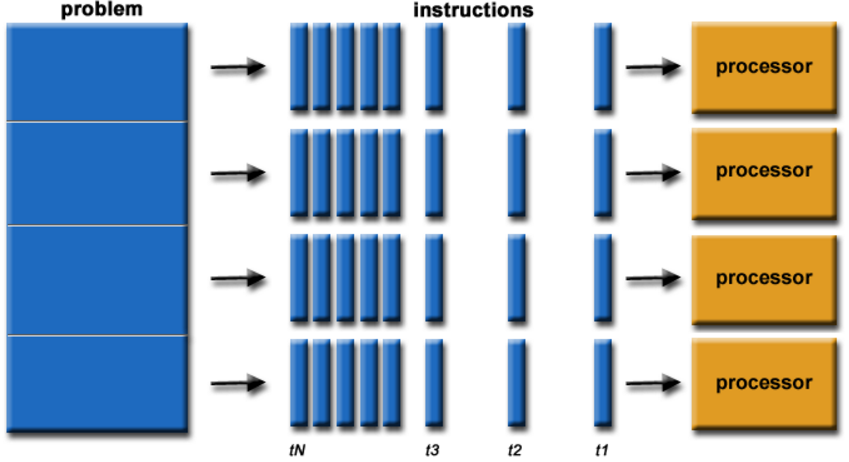
\includegraphics[width = 0.45\textwidth]{par_prob}}
    
    \caption{Serial and parallel computation of a problem}

\end{figure}

A typical parallel architecture is composed by an arbitrary number of computers, called \textit{nodes}, each of them with multiple processors, cores, functional units, ect. connected all together by a network:

\begin{figure}[H]

    \centering
    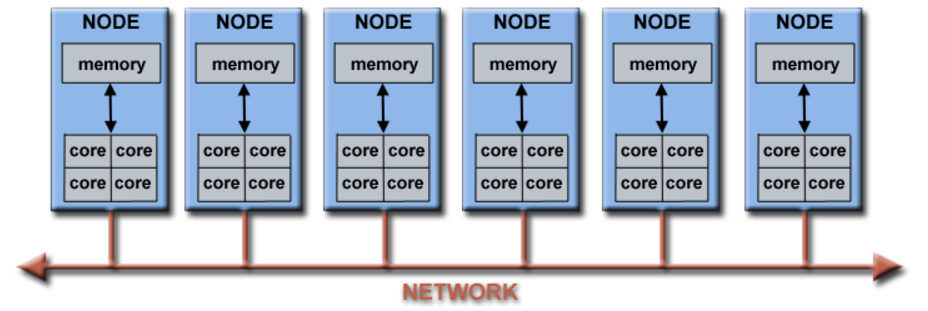
\includegraphics[width = 0.8\textwidth]{par_net}
    \caption{Parallel architecture schema}

\end{figure}

Inside a parallel architecture there can be heterogeneous nodes, with different computing techniques and configurations; according to Flynn's classical taxonomy, we can identify four different ways to classify computing architectures: 

\begin{enumerate}

    \item \textit{Single Instruction, Single Data (SISD)}: this is the original kind of computer, in which there is only one instruction stream that is managed by the Central Processing Unit (CPU) during clock cycles; this is serial, so non-parallel, computing. Figure \ref{fig::sisd} shows a SISD execution example, in which every instruction is executed after the previous one:
    
    \begin{figure}[H]

        \centering
        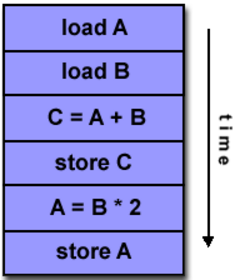
\includegraphics[width = 0.3\textwidth]{sisd}
        \caption{Instruction execution in a SISD architecture example}
        \label{fig::sisd}
    
    \end{figure}
    
    \item \textit{Single Instruction, Multiple Data (SIMD)}: at any clock cycle, there is one instruction that is executed, but the processing units can operate on different data elements of the instruction; in figure \ref{fig::simd} a classical SIMD execution is shown, where vector \textit{A} and \textit{B} data are used to simultaneously modify vector \textit{C}:
    
    \begin{figure}[H]

        \centering
        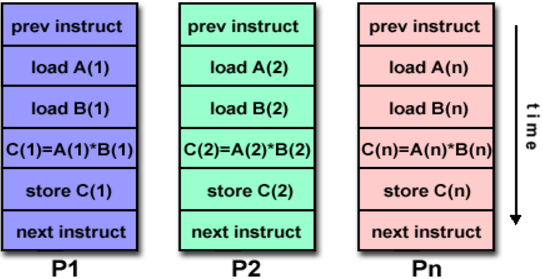
\includegraphics[width = 0.8\textwidth]{simd}
        \caption{Instruction execution in a SIMD architecture example}
        \label{fig::simd}
    
    \end{figure}
    
    \item \textit{Multiple Instruction, Single Data (MISD)}: a single data stream is managed by multiple processing units, that can independently operate on data through separate instruction streams; figure \ref{fig::misd} shows a MISD execution, where \textit{A(1)} is simultaneously used to compute different tasks:
    
    \begin{figure}[H]

        \centering
        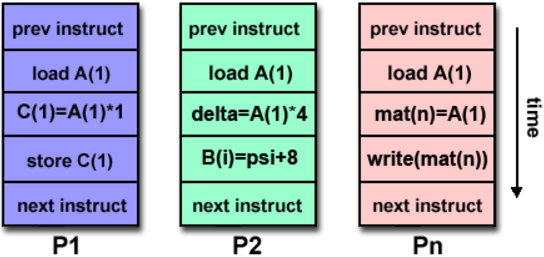
\includegraphics[width = 0.8\textwidth]{misd}
        \caption{Instruction execution in a MISD architecture example}
        \label{fig::misd}
    
    \end{figure}
    
    \item \textit{Multiple Instruction, Multiple Data (MIMD)}: every processing unit can execute different data and instruction streams; in figure \ref{fig::mimd}, processors concurrently elaborate different tasks that involve different elements:
    
    \begin{figure}[H]

        \centering
        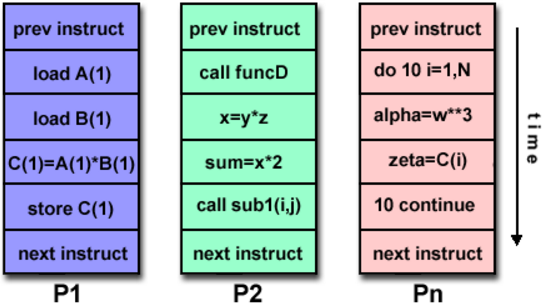
\includegraphics[width = 0.8\textwidth]{mimd}
        \caption{Instruction execution in a MIMD architecture example}
        \label{fig::mimd}
    
    \end{figure}

\end{enumerate}

Nowadays, among the introduced alternatives, MIMD architectures are the most used in parallel computing, especially in HPC systems.





\section{Design Space Exploration}

In many engineering problems there are several objectives that have to be obtained, with the presence of certain constraints and with the possibility to manage some customizable parameters; objectives can involve various metrics of interest, for instance connected to application throughput, system consumed power or overall cost.

Design Space Exploration (DSE) analyzes, in a systematic way, the space of possible parameters combinations that constitute application Design Space, with the objective to find the best design point that fulfills problem goals and requirements.

HPC applications have almost always a lot of parameters and related set of values, making the list of program configurations very long; in these cases the corresponding Design Space literally explodes, making impossible to analyze it in an exhaustive way.

\subsection{Multi-Objective Optimization (MOO) problem}

When there is more than one objective function that has to be accomplished, DSE consists of a Multi-Objective Optimization (MOO) problem; taking \cite{caramia2008multi} as reference, in mathematical terms a MOO problem can be defined as:

\begin{equation}
        min( f_1(x), f_2(x), ..., f_k(x) ), \quad k \ge 2 \qquad s.t. \quad x \in X
\end{equation}

where \textit{k} denotes the number of objective functions and \textit{X} represents the feasible region, defined by some constraints functions (for instance, in an embedded architecture, the total area should not exceed a predetermined value). If some of the objective functions have to be maximized, they can be attributed to minimizing its negation.

Multi-Objective Optimization problem has a lot of analogies into a wide variety of situations and domains, even the most common ones: formerly the ancients, given a set of seeds and a plot of land, had to choose what, how and how much farm, in order to maximize the harvest profit and to minimize the required effort, simultaneously not exceeding a cost limit; airline companies want to augment the number of passengers on their airplanes, to increase safety, to enlarge autonomy of their vehicles by means of various technical, strategic and commercial choices; an undergraduate student would minimize his/her university career duration and maximize his/her exam average, with a predetermined time limit and with the possibility to choose some coursers than others.

As it can be understood, since some objectives are in contrast with other objectives, a unique solution doesn't exist; for instance, in a microcontroller, an objective focused on performance would definitely confront against a power consumption one: the best solution for one of them would be the worst for the other and conversely. So, the aim of Design Space Exploration is almost always to search for a meeting point, between all the goals and requirements, that fulfills the overall problem.

Since therefore the concept of unique optimal solution can't be applied, it is useful to introduce the notion of Pareto optimality; pareto optimal solutions are, essentially, those ones that can't be improved without degrading at least one objective function. So, a solution \textit{x\textsuperscript{1}} is said to \textit{(Pareto) dominate} a solution \textit{x\textsuperscript{2}} if:

\begin{equation}
\begin{cases}
        f_i(x^1) \le f_i(x^2) \quad \forall i \in \{1, 2, ..., k\} \\
        f_j(x^1) < f_j(x^2) \quad \textit{for at least one } j \in \{1, 2, ..., k\}
\end{cases}
\end{equation}

The set of Pareto optimal solutions is often called Pareto front, Pareto frontier or Pareto boundary.





\section{Design of Experiments}\label{doe}

When a Design Space of an application is huge and, consequently, there is no possibility to do an exhaustive search over all possible configurations, there is the need to take a subset of points of interest that represent as closely as possible system behavior.

Therefore, on the one hand there is the quality of representation, that should be reliable enough; on the other, the number of simulations to do, that should be small.

Taking \cite{natrella2013nist} as reference, among various DoE techniques that generate the initial set of design points to be analyzed, we can mention:

\begin{itemize}

    \item \textit{Full-Factorial DoE}: it is made by all possible combinations among parameters values, so all possible application configurations are picked up;
 
    \item \textit{2-Level Full-Factorial DoE}: suitable for designs with two or more parameters, this DoE picks up all possible combinations among the extreme values of all parameters.
    
    If, for instance, there are three tunable parameters:
    
    \begin{enumerate}
    
        \item Number of Processors $\in$ \{ 2, 4, 8, 16, 32 \};
        
        \item Number of Threads $\in$ \{ 1, 2, 3, 4, 5, 6, 7, 8 \};
        
        \item Cache size $\in$ \{ 2K, 4K, 8K, 16K, 32K \}.
    
    \end{enumerate}
    
    the design points will be: \hbox{$\langle$ \#processors, \#threads, cache size $\rangle$} $\in$
    
    \{ $\langle$ 2, 1, 2K $\rangle$, $\langle$ 32, 1, 2K $\rangle$, $\langle$ 2, 8, 2K $\rangle$, $\langle$ 32, 8, 2K $\rangle$, \hbox{$\langle$ 2, 1, 32K $\rangle$}, \hbox{$\langle$ 32, 1, 32K $\rangle$}, $\langle$ 2, 8, 32K $\rangle$, $\langle$ 32, 8, 32K $\rangle$ \};

    \item \textit{Face Centered Central Composite DoE with one Center Point}: also this DoE is appropriate for designs with two or more parameters; the list of its design points can be split in three sets:
    
     \begin{enumerate}
    
        \item A 2-Level Full-Factorial Design set;
        
        \item A Center Point, in which each value is the median value of the corresponding parameter;
        
        \item An Axial Points set, in which all the median and extreme values of each parameter are combined.
    
    \end{enumerate}
    
    Considering the example in the previous DoE, the final design points list would be: $\langle$ \#processors, \#threads, cache size $\rangle$ $\in$
    
    \{ $\langle$ 2, 1, 2K $\rangle$, $\langle$ 32, 1, 2K $\rangle$, $\langle$ 2, 8, 2K $\rangle$, $\langle$ 32, 8, 2K $\rangle$, $\langle$ 2, 1, 32K $\rangle$, \hbox{$\langle$ 32, 1, 32K $\rangle$}, $\langle$ 2, 8, 32K $\rangle$, $\langle$ 32, 8, 32K $\rangle$ \} $\cup$ 
    
    \{ $\langle$ 8, 4, 8K $\rangle$ \} $\cup$
    
    \{ $\langle$ 2, 4, 8K $\rangle$, $\langle$ 32, 4, 8K $\rangle$, $\langle$ 8, 1, 8K $\rangle$, $\langle$ 8, 8, 8K $\rangle$, $\langle$ 8, 4, 2K $\rangle$, \hbox{$\langle$ 8, 4, 32K $\rangle$} \};
    
    \item \textit{Plackett-Burman DoE}: this DoE might be useful to analyze, more eonomically, a larger number of variables; in fact, Plackett-Burman reduces the number of potential factors, constructing very economical designs with the number of points multiple of 4 (rather than power of 2, as in the 2-Level Full-Factorial DoE).
    
    Concerning the example above, in this case the final design points list would be: $\langle$ \#processors, \#threads, cache size $\rangle$ $\in$
    
    \{ $\langle$ 2, 1, 32K $\rangle$, $\langle$ 32, 1, 2K $\rangle$, $\langle$ 2, 8, 2K $\rangle$, $\langle$ 32, 8, 32K $\rangle$ \};
    
    \item \textit{Latin-Hypercube DoE}: this DoE randomly chooses parameters values for each design point; the number of final configurations can be set up in advance.

\end{itemize}





\section{Dynamic autotuning}

When applications expose some configurable parameters (also known as \textit{dynamic knobs}), the concept of dynamic autotuning is defined as the ability to find the best set of knobs values, in an automatic and systematic way, that satisfies application goals and requirements at runtime, properly reacting to possible objective functions change. For instance, a web video streaming application would be able to manage video quality according to the overload of its servers: in some situations, it could set up itself for the best possible resolution; sometimes, it should reduce quality in order to make still available its services to all connected clients.

IBM research studies on \textit{Autonomic Computing} (\cite{kephart2003vision}, \cite{computing2006architectural}) made a breakthrough on the concept of self-adapting systems that are able to manage themselves and to dynamically optimize their execution configuration at runtime; \textit{Autonomic Computing} is based of the MAPE-K control loop, showed in figure \ref{fig::mape-k}:

\begin{figure}[H]

    \centering
    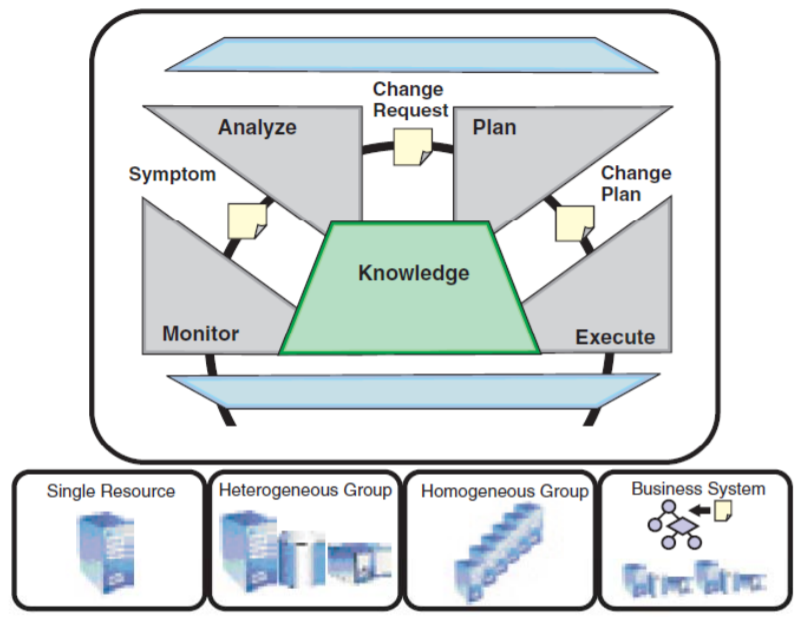
\includegraphics[width = 0.8\textwidth]{MAPE-K}
    \caption{MAPE-K control loop design}
    \label{fig::mape-k}

\end{figure}

In this control loop we can identify four principal functions:

\begin{itemize}

    \item \textit{Monitor}: it gathers application information about knobs setting and the associated metrics of interest values as, for instance, throughput and consumed power;
    
    \item \textit{Analyze}: it performs data analysis and reasoning on the information provided by the monitor function;
    
    \item \textit{Plan}: it reacts to a possible application objectives change during execution and it structures the actions needed to achieve this new state;
    
    \item \textit{Execute}: it modifies the behavior of the managed resource, according to the actions recommended by the plan function.

\end{itemize}

Finally, \textit{Knowledge} source is composed by all data that is used by the autonomic manager’s four functions; it includes information such as, for instance, topology structure, historical logs, metrics and policies.

Online autotuning therefore entrusts systems management from people to technology, achieving self-configuration and self-optimization objectives; applications requirements may change during execution and the overall system is able to react properly and to re-adapt itself.





\section{MQTT messaging protocol}\label{mqtt}

MQTT (Message Queue Telemetry Transport, \cite{banks2014mqtt}) is a lightweight messaging protocol that gives the possibility to establish remote communications among subjects. Its main characteristics are the minimization of network bandwidth and devices requirements but also the attention to the assurance of delivery; this features made MQTT ideal for machine-to-machine (M2M) or Internet of Things (IoT) world of connected devices, but in general this protocol have had a large use in different projects: for instance, the famous Facebook Messenger is built on top of it (\cite{zhang2011building}).

MQTT uses a client server publish\slash{}subscribe pattern: a client has the possibility to subscribe to topics and to publish messages on them (both topics and messages are strings); another component, called \textit{broker} server, deals with the dispatch of messages to only those clients that have subscribed to corresponding topics; so, publishers (those clients that sends messages) and subscribers (those clients that receive messages) don't know about the existence of one another: the broker, which is known by every client, will distribute messages accordingly. Figure \ref{fig::mqtt_example} shows a possible MQTT scenario with a sensor and two devices:

\begin{figure}[H]

    \centering
    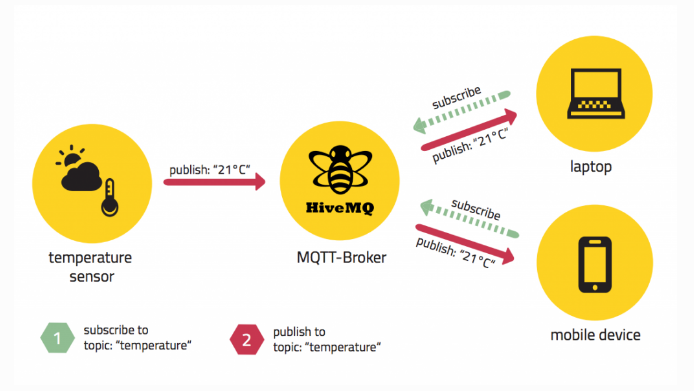
\includegraphics[width = 0.8\textwidth]{mqtt}
    \caption{MQTT publish/subscribe example, taken from \cite{site:hivemq}}
    \label{fig::mqtt_example}

\end{figure}

Topics are used by the broker to filter messages and manage them in a correct way; they are made up of one or more levels, separated by a forward slash, as shown in figure \ref{fig::topic}:

\begin{figure}[H]

    \centering
    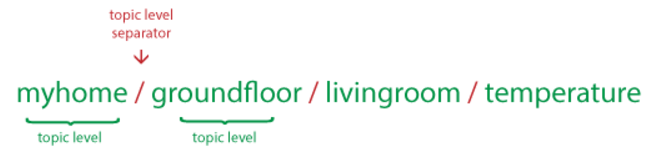
\includegraphics[width = 0.8\textwidth]{mqtt_toplevs}
    \caption{MQTT topic example, taken from \cite{site:hivemq}}
    \label{fig::topic}

\end{figure}

There is the possibility to subscribe to more topics at once through the use of wildcards: the single-level one (denoted with the symbol \textit{+}) and the multi-level one (indicated with the symbol \textit{\#}).

Single-level wildcard substitutes an arbitrary level in a topic, so all topics that matches the same structure will be associated to the one with single-level wildcard:

\begin{figure}[H]

    \centering
    
\includegraphics[width = 0.8\textwidth]{mqtt_singlew}
    \caption{MQTT topic with single-level wildcard example, taken from \cite{site:hivemq}}
    \label{fig:mqtt_singlew}

\end{figure}

for instance, \textit{myhome\slash{}groundfloor\slash{}kitchen\slash{}temperature} and \textit{myhome\slash{}\linebreak groundfloor\slash{}livingroom\slash{}temperature} will match the topic in figure \ref{fig:mqtt_singlew}, while \textit{myhome\slash{}groundfloor\slash{}kitchen\slash{}humidity} won't.

Multi-level wildcard is placed at the end of a topic and it covers an arbitrary number of topic levels:

\begin{figure}[H]

    \centering
    
\includegraphics[width = 0.8\textwidth]{mqtt_mulw}
    \caption{MQTT topic with multi-level wildcard example, taken from \cite{site:hivemq}}
    \label{fig:mqtt_mulw}

\end{figure}

in this case, for instance, \textit{myhome\slash{}groundfloor\slash{}kitchen\slash{}temperature} and \textit{myhome\slash{}groundfloor\slash{}kitchen\slash{}humidity} will match the topic in figure \ref{fig:mqtt_mulw}, while \textit{myhome\slash{}firstfloor\slash{}livingroom\slash{}temperature} won't.

Another interesting MQTT feature is the Last Will and Testament (LWT): each client can specify a normal MQTT message with topic and payload. When it connects to the broker, this message is stored; if client abruptly disconnects, the broker sends the corresponding LWT to all subscribed clients on related topic, notifying the occurred disconnection.





\section{Apache Spark\texorpdfstring{$^{TM}\;$}MMLlib library}

Agorà takes advantage of the Machine Learning MLlib library by Apache Spark\textsuperscript{TM} (\cite{spark2015apache}) in order to predict the complete model of running applications; in particular, it has been focused on the Generalized Linear Regression interface.


\subsection{(Generalized) Linear Regression}

Taking \cite{site:caltechML2012} as reference, Linear Regression tries to model the relationship between a variable \textit{y} and one or more variables \textit{x\textsubscript{1}, x\textsubscript{2}, ... x\textsubscript{n}, n $\ge$ 1}; more rigorously, given a set of statistical units $\{y_i, x_{i1}, x_{i2}, ..., x_{ip}\}_{i = 1}^n$, in which $y_i$ is the variable that depends on the p-vector $[x_{i1}, x_{i2}, ..., x_{ip}]$, linear regression assumes that this relationship is linear:

\begin{equation}
    y_i = \beta_0\boldsymbol{1} + \beta_1x_{i1} + \beta_2x_{i2} + ... +  \beta_px_{ip} + \epsilon_i, \quad i = 1, 2, ... n
\end{equation}

$y_i$ is the \textit{regressand}, \textit{endogenous variable}, \textit{response variable}, \textit{measured variable}, \textit{criterion variable} or \textit{dependent variable};

$x_{i1}, x_{i2}, ..., x_{ip}$ are called \textit{regressors}, \textit{exogenous variables}, \textit{explanatory variables}, \textit{covariates}, \textit{input variables}, \textit{predictor variables} or \textit{independent variables};

$\beta_0, \beta_1, ..., \beta_p$ are the \textit{effects} or \textit{regression coefficients}, whose values establish the connection between the regressand and the regressors; $\beta_0$ is also called \textit{intercept}; linear regression mainly focuses on the estimation of these parameters;

$\epsilon_i$ is called the \textit{error term}, \textit{disturbance term} or \textit{noise}. It represents all other factors that influence $y_i$ other than the predictor variables.

Linear Regression assumes that the response variable follows a Gaussian distribution; Generalized Linear Regression (GLR) gives the possibility to specify other distributions taken from the exponential family; it is useful for several kinds of prediction problems including Linear Regression, Poisson Regression (for count data) and Logistic Regression (for binary data); moreover, GLR gives the possibility to specify a link function \textit{g} that relates the mean of the measured variable to the exogenous variables. In the case of Gaussian distribution for Linear Regression, the link function can be equal to \textit{Identity}, \textit{Log} and \textit{Inverse}, with an explicit meaning.


\subsection{Regressors transformations}\label{regrTransforms}

In order to use Linear Regression even if the relationship between the dependent variable and the independent variables is not linear, there is the necessity to modify the input variables; Agorà implements two possible regressors transformations:

\begin{enumerate}

    \item it transforms parameters values with inverse, square root and natural logarithmic functions; in union with the unaltered predictor variables, it tries to find the best model combining these transformations and the available link functions;
    
    \item it transforms parameters values through the polynomial expansion of second order: their cross-products and square values are added to the set of regressors, evaluating the best model with the available link functions.

\end{enumerate}

Agorà chooses the model with the smallest Akaike Information Criterion (AIC) value, that is a measure of the quality, in terms of lost information, of statistical models for a given set of data; at the same AIC value, the chosen model is the one with the smallest mean of the sum of coefficient standard errors, that measure how precisely the model has estimated the regression coefficients with the given training set of data.




\section{Thesis structure}

\textit{ [Da fare in ultimo, quando tutta la struttura della tesi è chiara] }
